\documentclass{article}

\usepackage{graphicx}
\usepackage{tikz}
\usepackage{tikzsymbols}
\usetikzlibrary{calc,patterns,shapes.geometric}
\pagestyle{empty}
\usepackage[margin=0pt]{geometry}
\geometry{papersize={14in,12in}}

\def\centerarc[#1](#2)(#3:#4:#5){\draw[#1] ($(#2)+({#5*cos(#3)},{#5*sin(#3)})$) arc (#3:#4:#5);}

\begin{document}
	\begin{figure}
		\centering
		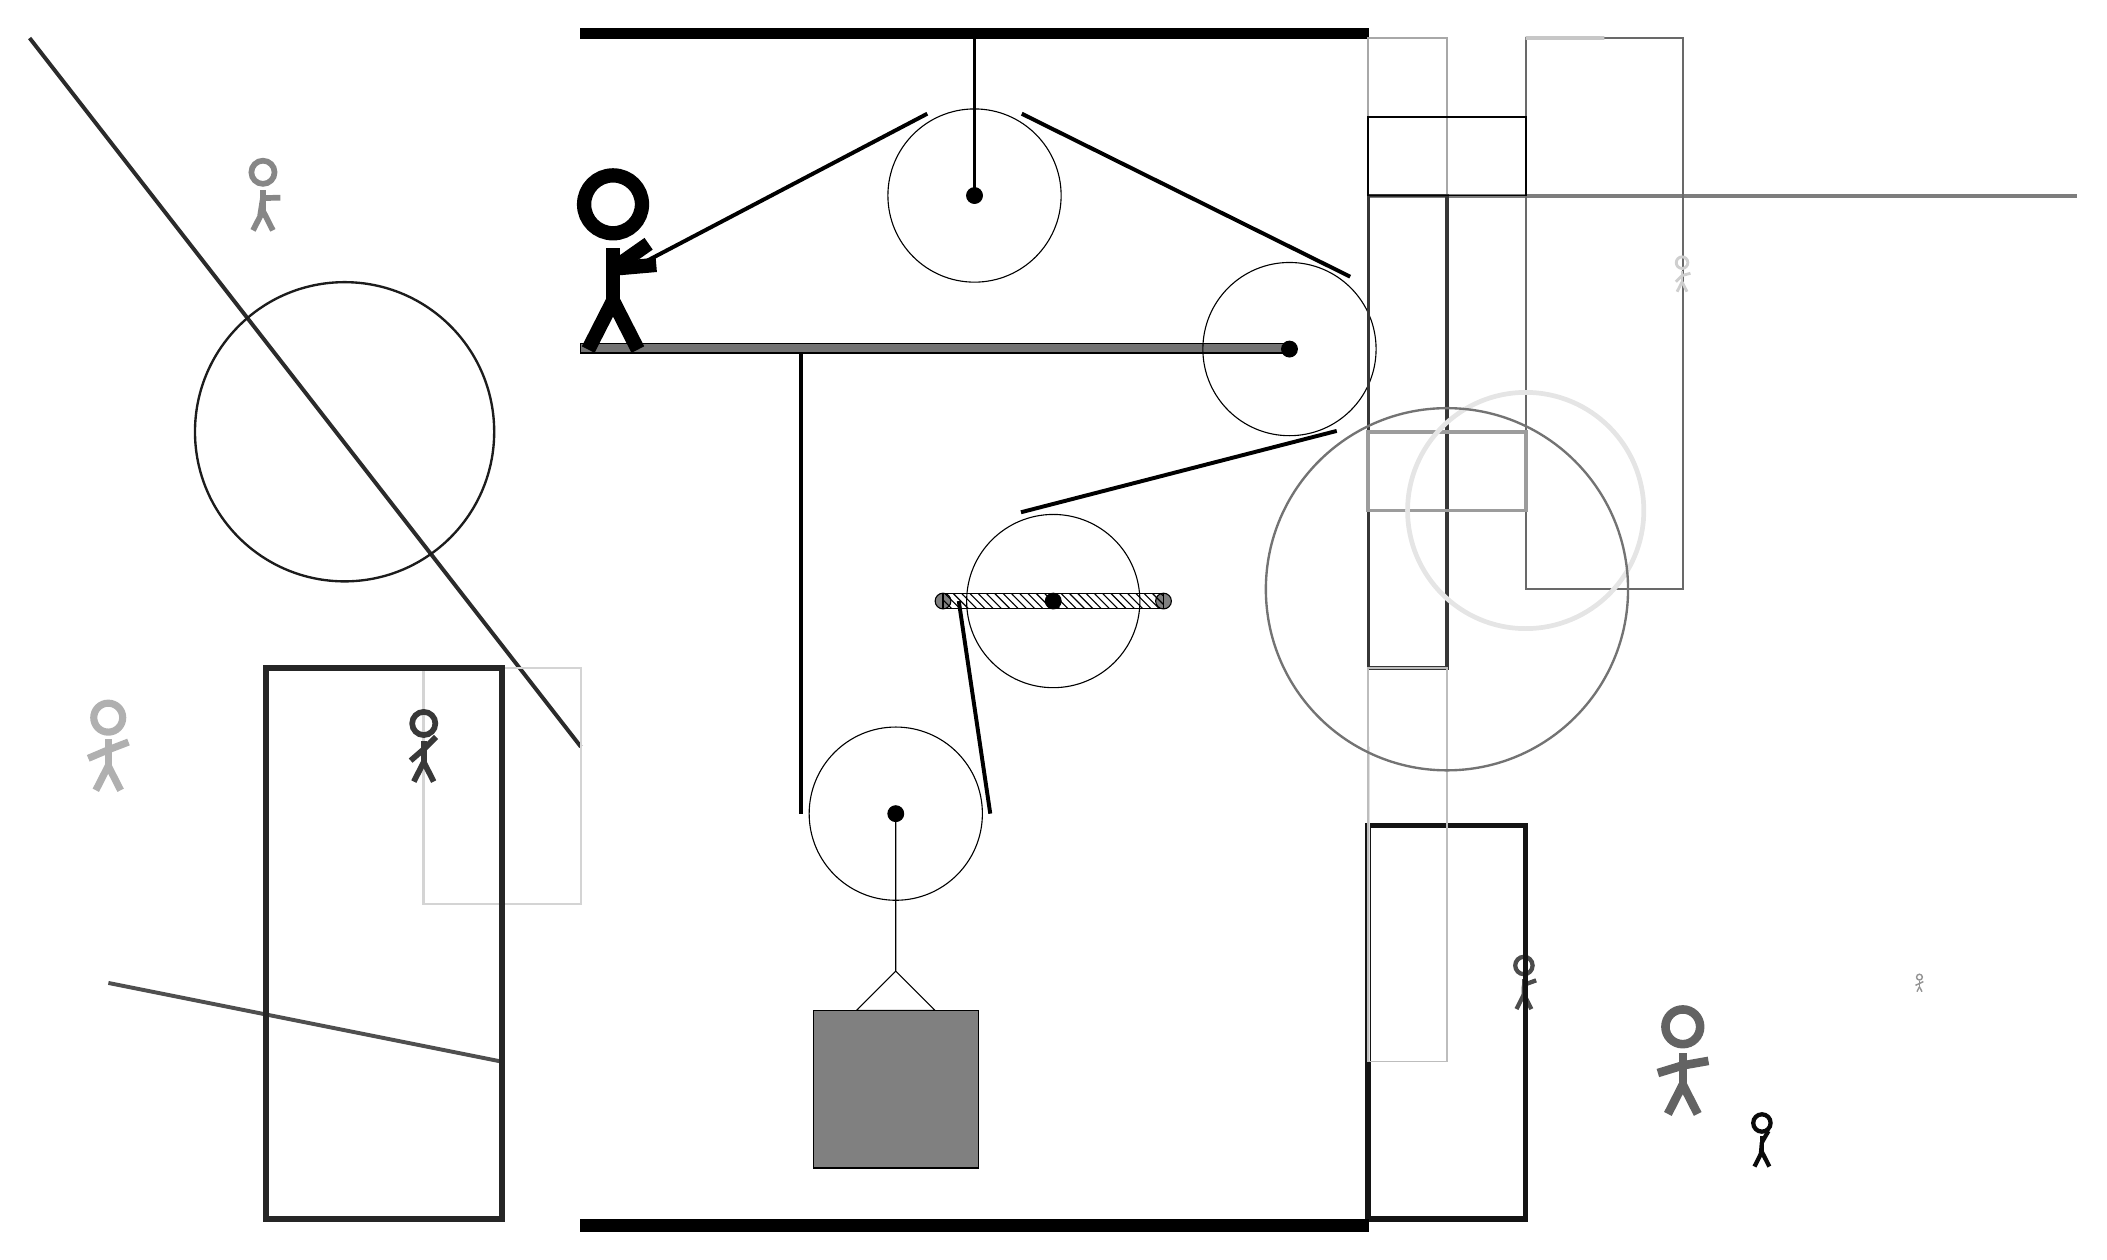
\begin{tikzpicture}
			%%%%% START %%%%%
			
			\draw[fill=black] (-2, 13) rectangle (8, 13.125);
			
			\draw[fill=black!55] (-2, 9) rectangle (7, 9.125);
			
			\draw (2, 3.15) circle (1.1);
			\draw[fill=black] (2, 3.15) circle (0.1);
			
			\draw (7, 9.05) circle (1.1);
			\draw[fill=black] (7, 9.05) circle (0.1);
			
			\draw[line width=0.5mm, color=black!69](-3, 0) -- (-8, 1);
			
			\draw[line width=0.5mm, color=black!51](8, 11) -- (17, 11);
			\draw[line width=0.3mm, color=black!34] (8, 11) rectangle (9, 13);
			\draw[line width=0.5mm, color=black!83](-2, 4) -- (-9, 13);
			
			\draw[line width=0.3mm, color=black!59] (10, 6) rectangle (12, 13);
			
			\draw[line width=0.3mm, color=black!17] (-4, 2) rectangle (-2, 5);
			\draw[line width=0.4mm, color=black!79] (8, 11) rectangle (9, 5);
			
			\node[line width=0.6mm, color=black!70] at (10, 1) {\Strichmaxerl[3][89][20]};
			\node[line width=0.2mm, color=black!61] at (12, 0) {\Strichmaxerl[6][17][10]};
			
			\node[line width=0.6mm, color=black!31] at (-8, 4) {\Strichmaxerl[5][23][21]};
			\node[line width=0.5mm, color=black!96] at (13, -1) {\Strichmaxerl[3][85][60]};
			
			\draw [line width=0.3mm, color=black!89](-5, 8) circle (1.9);
			\node[line width=0.5mm, color=black!42] at (15, 1) {\Strichmaxerl[1][24][27]};
			
			\draw[line width=0.5mm, color=black!39] (8, 7) rectangle (10, 8);
			\node[line width=0.6mm, color=black!19] at (12, 10) {\Strichmaxerl[2][45][15]};
			\draw[line width=0.7mm, color=black!85] (-3, -2) rectangle (-6, 5);
			\draw[line width=0.2mm, color=black!99] (10, 11) rectangle (8, 12);
			\draw [line width=0.6mm, color=black!10](10, 7) circle (1.5);
			\draw[line width=0.7mm, color=black!92] (10, 3) rectangle (8, -2);
			\draw[line width=0.4mm, color=black!12] (8, 4) rectangle (8, 0);
			\draw[line width=0.4mm, color=black!22] (10, 13) rectangle (11, 13);
			\node[line width=0.2mm, color=black!78] at (-4, 4) {\Strichmaxerl[4][41][45]};
			
			\node[line width=0.3mm, color=black!47] at (-6, 11) {\Strichmaxerl[4][81][1]};
			\draw[line width=0.2mm, color=black!26] (9, 5) rectangle (8, 0);
			\draw [line width=0.3mm, color=black!55](9, 6) circle (2.3);
			
			\draw[fill=white](4, 5.85) circle (1.1);
			\draw[fill=black] (4, 5.85) circle (0.1);
			\draw[fill=black!50] (2.6, 5.85) circle (0.1);
			\draw[fill=black!50] (5.4, 5.85) circle (0.1);
			\draw[pattern=north west lines, pattern color=black] (2.6, 5.95) rectangle (5.4, 5.75);
			
			\draw (3, 11) circle (1.1);
			\draw[fill=black] (3, 11) circle (0.1);
			\draw[line width=0.5mm] (3, 11) -- (3, 13);
			
			\draw (2, 3.15) -- (2, 1.15) -- (1.5, 0.65) -- (2.5, 0.65) -- (2, 1.15);
			\draw[fill=black!50] (0.95, 0.65) rectangle (3.05, -1.35);
			
			\draw[line width=0.5mm] (0.8, 9) -- (0.8, 3.15);
			\centerarc[line width=0.5mm](2, 3.15)(180:360:1.2000000000000002);
			\draw[line width=0.5mm](3.2, 3.15) -- (2.8, 5.85);
			\centerarc[line width=0.5mm](4, 5.85)(110:180:1.2000000000000002);
			\draw[line width=0.5mm](3.5896, 6.9776) -- (7.6, 8.0108);
			\centerarc[line width=0.5mm](7, 9.05)(-60:50:1.2000000000000002);
			\draw[line width=0.5mm](7.7714, 9.9692) -- (3.6, 12.0392);
			\centerarc[line width=0.5mm](3, 11)(60:120:1.2000000000000002);
			\draw[line width=0.5mm](2.4, 12.0392) -- (-1.2, 10.15);
			
			\node at (-1.5, 10.15) {\Strichmaxerl[10][-175][35]};
			
			\draw[fill=black] (-2, -2) rectangle (8, -2.15);
			
			%%%%% END %%%%%
		\end{tikzpicture}
	\end{figure}	
\end{document}